\section{Methods}
\textbf{Pre-processing.} We applied the DICOM rescale slope and intercept, inverted MONOCHROME1 images, normalised each image to 8 bit by its own minimum and maximum, replicated it to three channels and resized it to 224 pixels (Swin-T) or 256 pixels (all others). ImageNet mean and standard deviation were used for scaling.
\textbf{Models.} All backbones were ImageNet-pretrained timm models (Swin-T, DenseNet121, EfficientNetV2-S, ConvNeXt-T, ResNet50, EfficientNet-B3), each with a 22-way sigmoid head and a 22-way softmax head. For the fusion ablation we combined DenseNet121 and Swin-T in five ways: a learned gate on raw features, the same gate with LayerNorm, a fixed 0.5/0.5 average, the CNN branch alone, and the Swin branch alone.
\textbf{Training.} We used AdamW (weight decay 1e-4; learning rate 2e-4 for Swin, 3e-4 for DenseNet, ResNet and EfficientNet, 1e-4 for ConvNeXt), a cosine schedule with one warm-up epoch, 30 epochs, batch size 32, fp16, an exponential moving average of the weights (0.998) and gradient clipping at 5. The loss was binary cross-entropy with positive weights capped at 20, plus 0.5 times a soft-target cross-entropy on the softmax head. Light augmentation was flip, shift-scale-rotate and brightness/contrast; heavy augmentation added noise and blur. We did not pick checkpoints: the final averaged weights were used.
\textbf{Decisions made on out-of-fold (OOF) predictions only.} These were the head and test-time-augmentation variant of each run, the ensemble weights (greedy Caruana selection, 40 iterations), the per-class thresholds (coordinate ascent on sample-mean F1, shrunk towards 0.5 with weight n\_pos/(n\_pos+20)) and the rule that every image gets at least one label. The held-out set was used once (Fig. 1).
\begin{figure}[htbp]\centering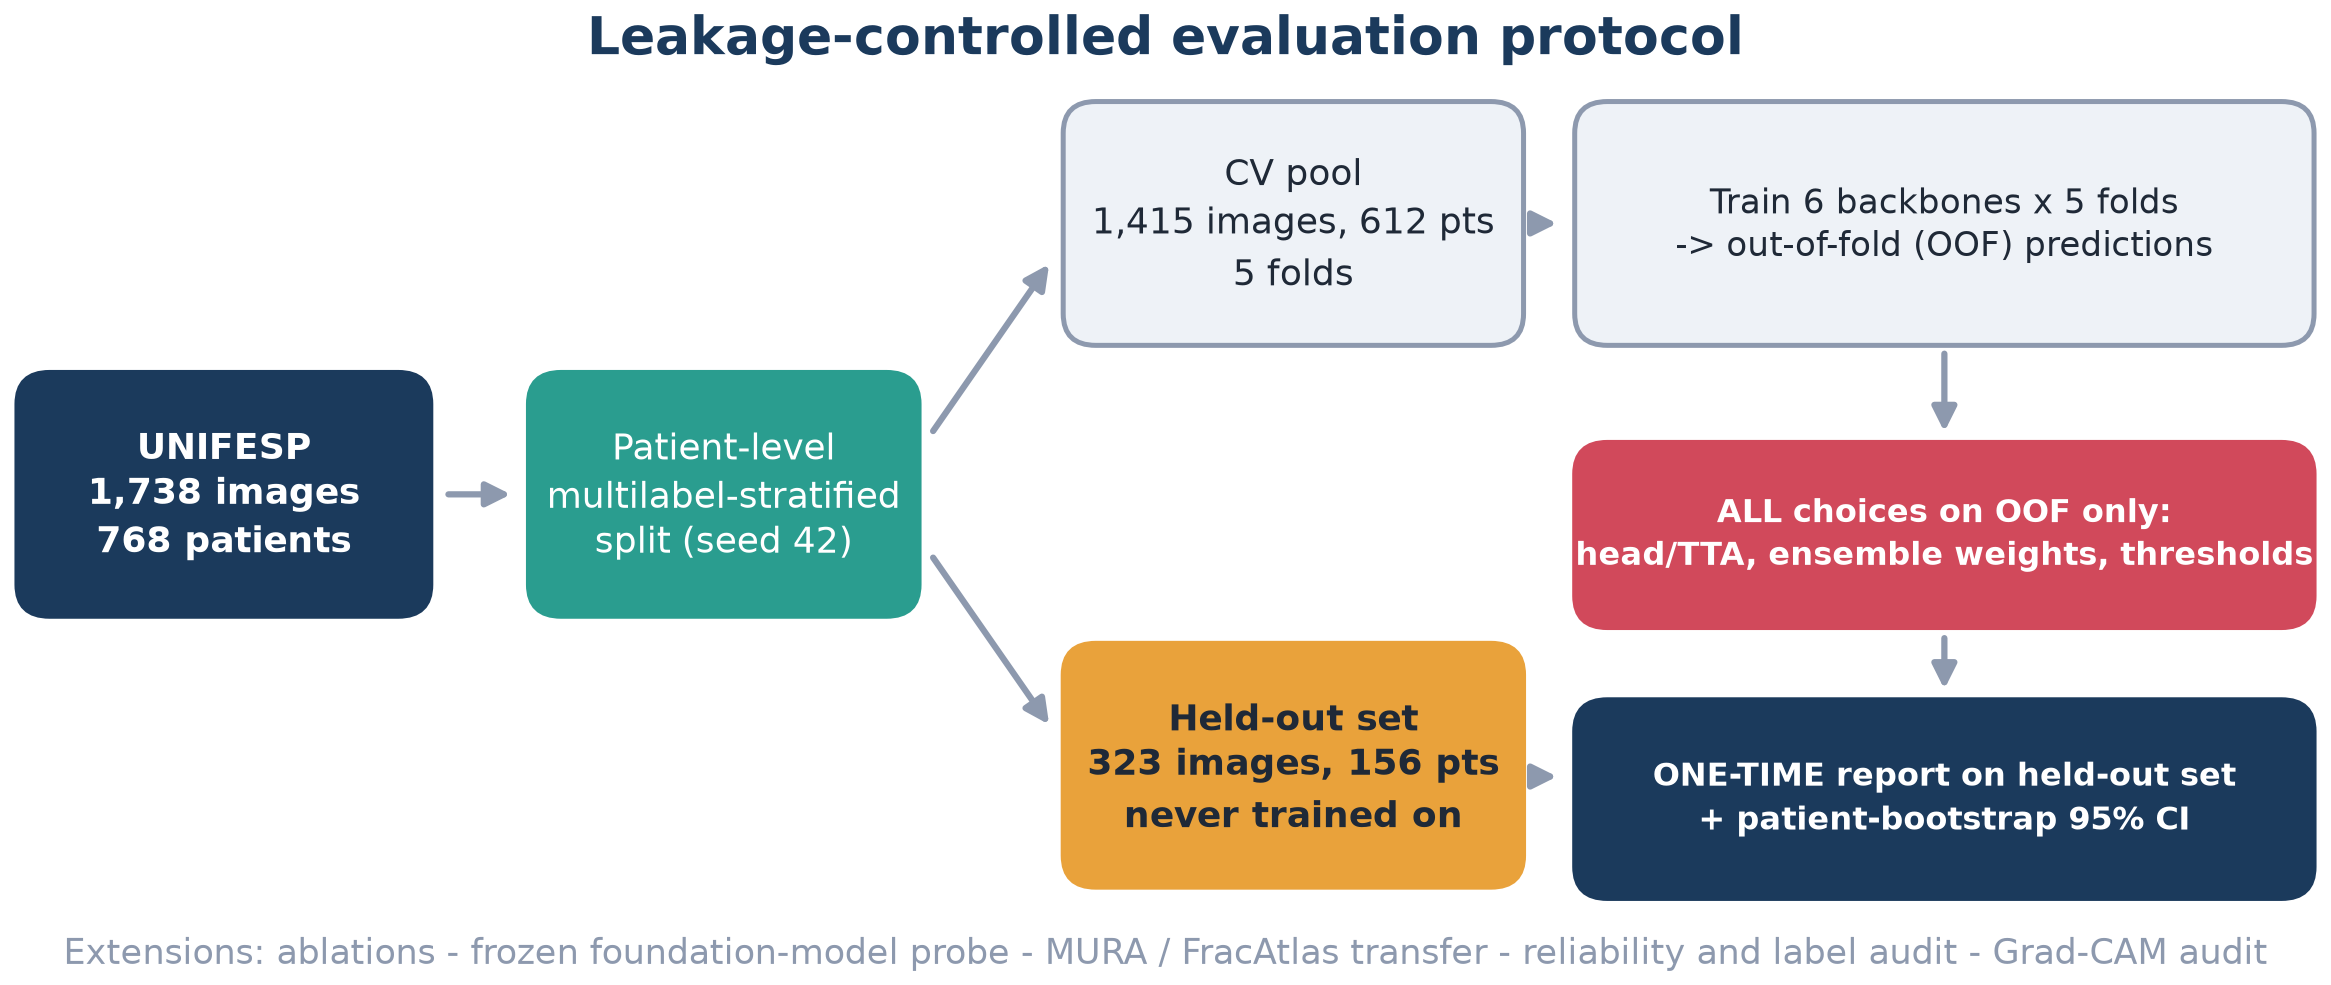
\includegraphics[width=0.95\textwidth]{fig1_protocol.png}\caption{Evaluation protocol. Images are split by patient into a cross-validation pool and a held-out set. Every choice is made on out-of-fold predictions, and the held-out set is scored once, with patient-bootstrap confidence intervals.}\label{fig:1}\end{figure}

\textbf{Metrics and statistics.} We report sample-mean F1 (the competition metric), macro-F1, micro-F1 and subset accuracy. Confidence intervals are 95 \% patient-level bootstrap intervals (2,000 resamples, or 1,000 for the reliability analysis), and model comparisons use a paired patient bootstrap. FracAtlas and the other transfer targets have no patient identifiers, so their intervals come from an image-level bootstrap and are optimistic.
\textbf{Frozen foundation-model baseline.} We froze DINOv2-S, DINOv2-B and an ImageNet Swin-T at 224 pixels, standardised the features on the cross-validation pool and trained a linear probe with 22 sigmoid outputs (binary cross-entropy plus L2). Weight decay was chosen on OOF predictions, and folds and held-out set were the same as before. To get a label-efficiency curve we repeated this with 10, 25, 50 and 100 \% of the training patients in each fold.
\textbf{Cross-dataset transfer.} We mapped the label spaces onto each other in a closed set (for example MURA hand, wrist and forearm onto the UNIFESP classes of the same name), restricted predictions to the shared groups and report accuracy and macro-F1. The map is our own assumption.
\textbf{Reliability analysis.} The ensemble combined five saved ablation runs (three Swin-T seeds, DenseNet121 and ConvNeXt-T) with weights fitted on OOF predictions. We measured top-1 calibration (ECE with 15 bins; temperature fitted on OOF, applied to the held-out set), drew a risk-coverage curve in which the model abstains on low-confidence images, and computed per-class precision, recall and F1 with patient bootstrap intervals. For the \textbf{label audit}, a training image counts as a \emph{suspect} when the OOF ensemble gives probability 0.9 or more to a class other than its given label and a low probability to the given one (as in confident learning). Suspects are not proven errors.
\textbf{Explainability.} We computed Grad-CAM maps for three fold-0 models on the held-out set, ran a deletion test against a random map on the same grid, and ran a randomisation sanity check.
\textbf{Hardware and software.} All runs used Kaggle notebooks on 2 $\times$ NVIDIA T4 GPUs (Stage 2 took 18,811 s) with PyTorch 2.11.0 (CUDA 13.0). The other libraries (timm, albumentations, pydicom, scikit-learn) were the versions preinstalled on the Kaggle image at the time of the runs, from October to November 2026; we did not record a full package list, which we list as a limitation. Code, split files and seeds are released on GitHub (Zenodo, doi:10.5281/zenodo.24027438).

